Robots operating in unstructured, stochastic environments such as a
factory floor or a kitchen face a difficult planning problem due to
the large state space and the very large set of possible
tasks~\citep{bollini12,knepper13}.  A powerful and flexible robot such
as a mobile manipulator in the home has a very large set of possible
actions, any of which may be relevant depending on the current goal
(for example, robots assembling furinture~\citep{knepper13} or baking
cookies~\citep{bollini12}.)  When a robot is manipulating objects in
an environment, an object can be placed anywhere in a large set of
locations.  The size of the state space increases exponentially with
the number of objects, which bounds the placement problems that the
robot is able to expediently solve.  Depending on the reward function
(which is unknown before runtime), any of these states and actions may
be relevant to the solution, but for any specific reward function,
most of them are irrelevant.  For instance, when making brownies, the
oven and flour are important, while the soy sauce and saut\'{e} pan
are not.  For a different task, such as stir-frying broccoli, the
robot must use a different set of objects and
actions. 
\begin{figure}
\centering
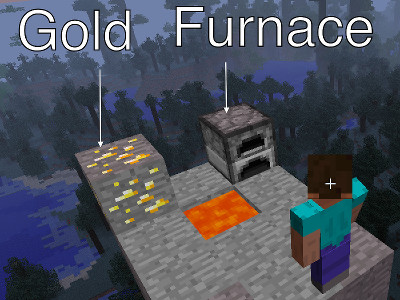
\includegraphics[width=0.49\linewidth]{figures/smelt_small.jpg}
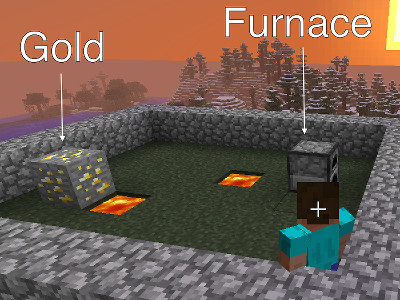
\includegraphics[width=0.49\linewidth]{figures/smelt_large.jpg}
\caption{Two different problems from the same domain, where the
  agent's goal is to smelt the gold in the furnace while avoiding the
  lava.  Our agent is unable to solve the problem on the right before
  learning because the state/action space is too large (since it can
  place the gold block anywhere).  After learning, it can quickly
  solve the larger problem.\label{fig:example}}
\end{figure}

To confront this state-action space explosion, prior work has explored
adding knowledge to the planner, such as options~\cite{sutton99} and
macro-actions~\cite{Botea:2005kx,Newton:2005vn}.  However, while these
methods can allow the agent to search more deeply in the state space,
they add non-primitive actions to the planner which {\em increase} the
branching factor of the state-action space.  The resulting augmented
space is even larger, which can have the paradoxical effect of
increasing the search time for a good policy~\cite{Jong:2008zr}.
Deterministic forward-search algorithms like hierarchical task
networks (HTNs)~\citep{Nau:1999:SSH:1624312.1624357}, and temporal
logical planning
(TLPlan)~\citep{Bacchus95usingtemporal,Bacchus99usingtemporal}, add
knowledge to the planner that greatly increases planning speed, but do
not generalize to stochastic domains. Additionally, the knowledge
provided to the planner by these methods is quite extensive, reducing
the agent's autonomy and must be manually supplied by the designer.

To address these issues, we augment an Object Oriented Markov Decision
Process (OO-MDP) with a specific type of action prior conditioned on
the current state and an abstract goal description.  Because we
condition on both the state and goal description, we refer to this
type of action prior as a knowlege base of {\em affordances}.
Affordances were originally proposed by \citet{gibson77} as action
possibilities prescribed by an agent's capabilities in an environment.
%Affordances focus an agent's attention on aspects of the environment that
%are most relevant to solving its current goal and avoid exploration of irrelevant parts of the
%world.
We rigorously formalize the notion of affordances as a prior on
actions conditioned on features of the current state as well as the
robot's goal.  Affordances enable the robot to prune irrelevant
actions on a state-by-state basis based on the agent's current goal
and focus on the most promising parts of the state space.  Affordances
can be specified by hand or alternatively learned through experience
in related problems, making them a concise, transferable, and
learnable means of representing useful planning knowledge. Our
experiments demonstrate that affordances provide dramatic improvements
for a variety of planning tasks compared to baselines in simulation,
and are applicable across different state spaces.  Moreover, while
manually provided affordances outperform baselines, affordances
learned through experience yield even greater improvements.We conduct
experiments in the game Minecraft, which has a very large state-action
space, and on a real-world robotic cooking assistant.
Figure~\ref{fig:example} shows an example of two problems from the
same domain in the game Minecraft; the agent learns on randomly
generated problems and tests on new problems from the same domain that
it has never previously encountered. 
